\documentclass[../handbook.tex]{subfiles}
\graphicspath{{\subfix{../pics/}}}
\begin{document}

\chapter{A\slash B-тестирование}

% The Plan: AA-tests
% 1. Splitting
% 2. SRM
% 3. Validate stat.criteria

\section{Ошибки, значимость, p-value}

\begin{margintable}
    \caption{Ошибки I-го и II-го рода}
    \label{tab:mistakes}
    \begin{center}
        \begin{tabular}[c]{c|c c}
            {\it гипотеза} & верна & не верна \\
            \hline
            принята & + & {\it II род} \\
            отвергнута & {\it I род} & + \\
        \end{tabular}
    \end{center}
\end{margintable}

Если мы хотим опровергнуть какое-то утверждение, мы должны сформулировать
альтернативную гипотезу. Основная гипотеза всегда обозначается $H_0$,
альтернативная $H_1$. Основная гипотеза всегда должна быть простой, каким-то
конкретным утверждением, альтернативная может быть каким угодно. Такое
требование создается потому, что у нас нет мат.аппарата на сложные условия.

Влиять мы можем только на ошибку I-го рода. Ее обычно фиксируют на уровне 0,05,
0,01 или 0,005, но этот уровень можно менять на любой другой если этого требует
задача.

Ошибки второго рода контролировать сложнее. Для их уменьшения стараются
пользоваться состоятельными критериями.\marginpar{Критерий проверки гипотезы
называется состоятельным, если ошибка второго рода уменьшается с ростом числа
наблюдений.}

\begin{marginfigure}
    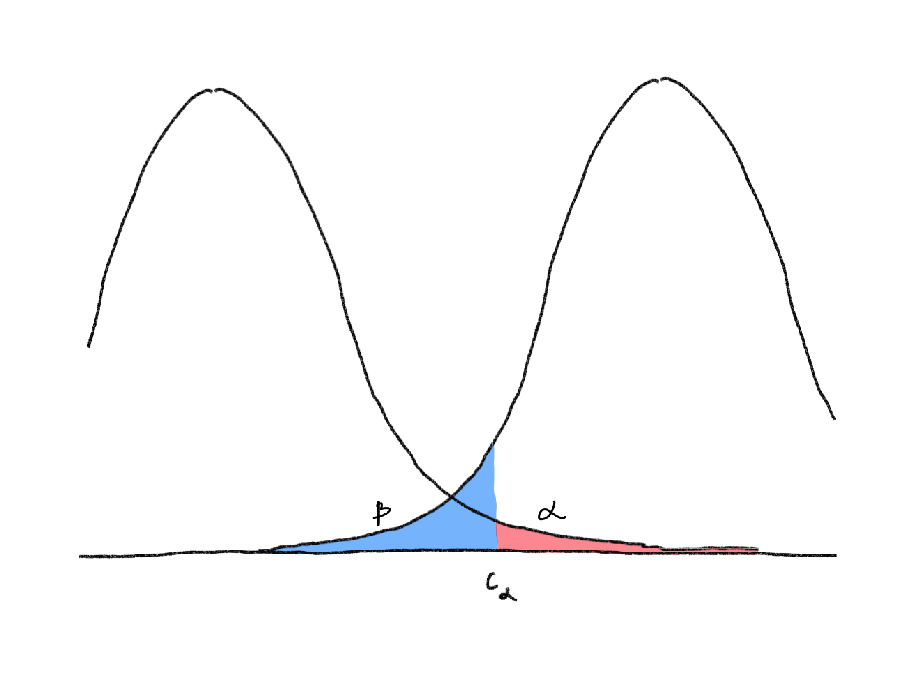
\includegraphics[width=1.1\columnwidth]{pics/critical_points_mistakes_value.pdf}
    \caption{Левое распределение соответствует гипотезе $H_0$, правое - гипотезе $H_1$.}
    \label{fig:crit_point}
\end{marginfigure}
Критическая точка критерия это такое значение вероятность превысить которое
равняется~$\alpha$ то есть вероятности ошибки первого рода. На рисунке
\ref{fig:crit_point} это площадь под графиком выше критической точки окрашенная
в красный. Синим обозначена вероятность ошибки II-го рода. Как видно это
вероятность получить выборку при которой не отвергается нулевая гипотеза, но
была верна альтернативная гипотеза.\marginpar{Проверять
    статистические гипотезы можно только в случае массовых явлений. События
    которые редки стат.гипотезами не проверяются. Число в 30 наблюдений
    считается достаточным только для нормальных распределений, для всех
    остальных надо больше данных.}

Критическая точка не обязана лежать на пересечении плотностей распределений
двух гипотез. Она определяется исходя только из плотности для нулевой гипотезы.

Альтернативой к механике проверки гипотез с критической точкой является
проверка гипотез через p-value. P-value вычисляется из предположения, что
нулевая гипотеза верна и определяет вероятность получить такое же значение
критерия или более экстремальное. Нам все равно нужно фиксировать уровень
значимости~$\alpha$ до эксперимента, но не нужно вычислять критическую точку.
Если p-value оказалось меньше~$\alpha$ то нулевая гипотеза должна быть
отвергнута, в противном случае нет оснований отвергать нулевую гипотезу.

\subsection{Ошибка подглядывания}
Ошибка подглядывания возникает когда мы заглядываем в результаты теста до
окончания самого теста (в промежуточное время). В этот момент человек может
увидеть промежуточный результат p-value~$< \alpha$. Во время подглядывания
может возникнуть соблазн дождаться когда p-value упадет ниже уровня
стат.значимости и остановить эксперимент. На самом деле график p-value в
процессе эксперимента может несколько раз опускаться ниже стат.значимости. Это
будет происходить случайно.\sidenote{\fullcite{karpov:ab_peeping}}

\marginpar{{\bf Процедура статистического тестирования:}
    \begin{enumerate}
        \item Определить метрику которую проверяем.
        \item Сформулировать нулевую и альтернативную гипотезы.
        \item Зафиксировать уровень стат.значимости~$\alpha$.
        \item Предрасчитать объем необходимой выборки для теста.
        \item Предрасчитать длительность теста.
        \item Запуск теста. В промежуточные результаты не заглядываем.
        \item По истечению времени, интерпретация результатов.
    \end{enumerate}

    Такая процедура обеспечит, что из всей массы запущенных экспериментов ошибки I рода будут наблюдаться с вероятностью~$\alpha$.
}

В случае если \emph{нулевая гипотеза верна}, вероятность получить p-value на
определенном уровне имеет равномерное распределение. Например, вероятность
получить p-value из первого дециля равна 10\%, вероятность получить p-value из
второго дециля это $P(\text{p-value} < 0.2) - P(\text{p-value} < 0.1) = 0.1$
тоже 10\%. Это означает, что отвергать нулевую гипотезу, то есть совершать ошибку I рода, мы будем с вероятностью~$\alpha$. 

Если же следить за p-value пока он не опустится ниже~$\alpha$ мы увеличим вероятность ошибки I рода и перестанем ее контролировать. И по сути будем выдавать желаемое за действительное.

\subsection{A/A-test}
Когда проверяются гипотезы статистикой, лучше провести
А/А-тес\-ти\-ро\-ва\-ние. Во время тестирования нужно просимулировать
что-нибудь и проверить как работают критерии которыми будет проверяться будущий
эксперимент.

Может оказаться так, что какие-то критерии не работают потому, что нарушаются
условия (каким-то неизвестным нам образом) применения этих критериев. В этом
случае A/A-тесты не сойдутся и это повод выяснить причины и устранить их до
запуска полноценного A/B-теста.

\section{Нормальность}
\marginpar{
    $\mu_k$ --- $k$-ый момент \\
    $\sigma$ --- ср.кв.отклонение
}
Проверять данные на нормальность стоит не слишком тщательно. Данным достаточно только \emph{напоминать} нормальные, чтобы использовать большинство критериев в которых подразумевается, что данные нормальные. Если подходить к проверкам строго, то ничто и никогда невозможно будет проверить. 

Точно необходимо проверить:
\begin{enumerate}
    \item Выбросы. Отсутствие выбросов достаточно критичное условие. Если в данных есть выбросы, то их нельзя считать нормальными. С другой стороны если эти выбросы убрать, возможно уже можно будет работать.

    
    \item Асимметрия.\marginnote{ \[A = \frac{\mu_3}{\sigma^3}\]}
        Нормальные данные должны быть симметричными, поэтому если наблюдается асимметрия, то данные не нормальные. Возможно сможет помочь логарифмирование. 

    \item Эксцесс (kurtosis) --- отклонение от колоколообразности.
        \marginnote{ \[\gamma_2 = \frac{\mu_4}{\sigma^4} - 3\]}
        Пограничным случаем колоколообразности можно считать равномерное распределение, а вот бимодальность гистограммы уже явный признак, что данные не нормальны. Еще чем больше наблюдений в данных, тем все-таки ближе должна быть гистограмма к нормальному распределению. За критерий можно взять выборку в $n=150$, чей график должен быть похож на колокол.
\end{enumerate}

Если в выборке менее 2000 объектов, то применяется метод Шапиро-Уилка, если же объектов больше, то используется критерий согласия Колмогорова-Смирнова.

\subsection{Удаление выбросов}
\paragraph{Преобразование Бокса-Кокса.} 
\marginpar{
    \begin{equation}
        \label{eq:box-cox}
        x_{i,\lambda} = 
        \begin{cases}
            \frac{x_i^\lambda - 1}{\lambda} & \text{если } \lambda \ne 0, \\
            \log(x_i) & \text{если } \lambda = 0.
        \end{cases}
    \end{equation}
}
это преобразование исходного набора
данных. Применяют в основном с целью устранения выбросов. Например,
при~$\lambda = 0$ это обычное логарифмическое преобразование.
Параметр~$\lambda$ подбирается методом оптимизации правдоподобия.

{\it Почему такая формула?} Логарифмическое преобразование хорошо себя
зарекомендовало, но оно не всегда справляется. Замечено, что $(\log x)' =
1/x$. Преобразование Бокса-Кокса это обобщение до функций чьи производные
равны $1/x^\lambda$.

\paragraph{Расстояние Махалонобиса.}
\marginpar{
    $m$ --- выборочный вектор мат.ожидания \\
    $S$ --- выборочная матрица ковариации
}
\begin{marginfigure}
    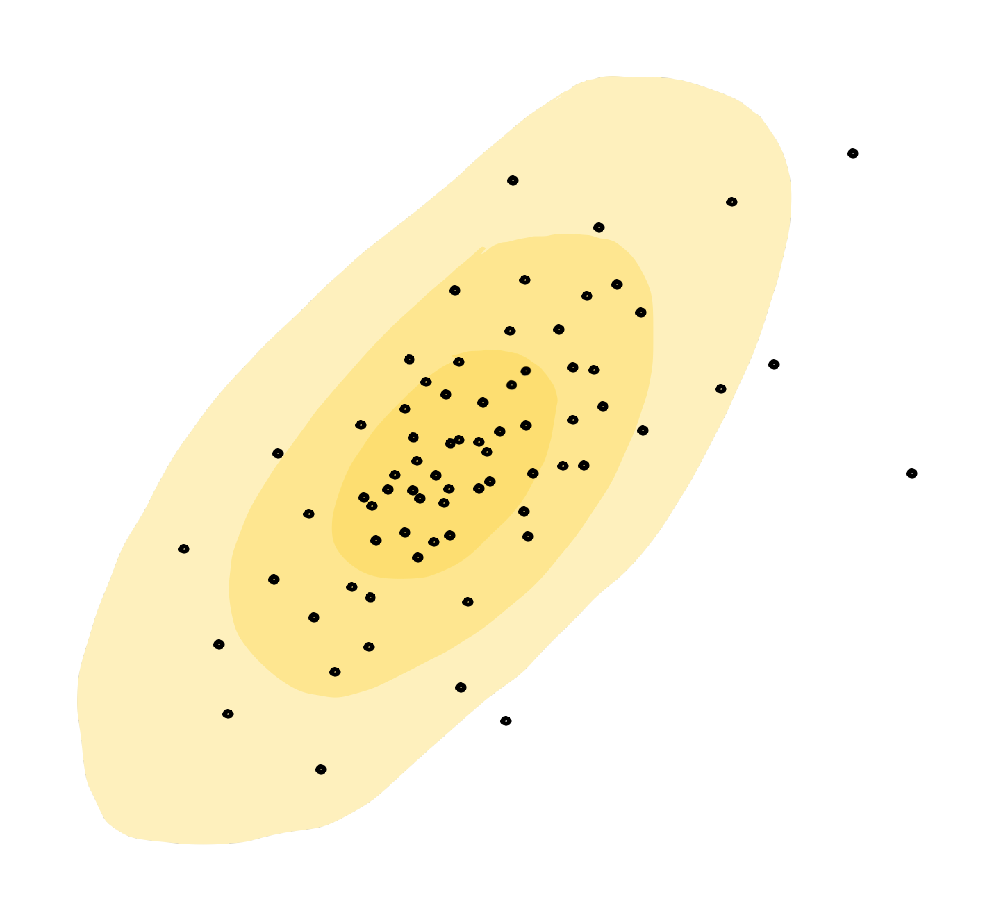
\includegraphics[width=0.8\columnwidth]{pics/mahalanobis.pdf}
    % \caption{выбросы через расстояние Махаланобиса}
    % \label{fig:mahalanobis}
\end{marginfigure}
Для многомерных данных можно предположить, что они распределены по какому-то многомерному нормальному закону распределения. Если центр (мат.ожидание) и матрицу ковариации для датасета, то можно определить расстояние Махалонобиса. Так мы получим аналог много\-мерной дисперсии и сможем вычислить отклонение от среднего
\begin{equation}
    \label{eq:mahalanobis}
    d = \sqrt{ (x - m) S^{-1}(x-m)^T}
\end{equation}
Мы можем использовать это расстояния для определения 95\% границы (или любой другой) чтобы построить область допустимых значений. Сэмплы за вычисленной границей будут считаться аутлайерами. Поскольку вычисление границы может оказаться дорогим, можно провести упрощенное действие: рассчитать для каждого сэмпла расстояние~\ref{eq:mahalanobis} и отрезать 5\% граничных квантилей.

\subsection{Бакетный тест}

\marginpar{
    $K = 30$ обычно достаточно, чтобы грубо оценить мат.ожидание
}
Если удаление выбросов не помогает сделать данные нормальными, например, есть выраженная асимметрия, то можно воспользоваться \emph{бакетным тестом}. Для этого разделим выборку на непересекающиеся подвыборки по $K$ элементов и измерим в каждой из них мат.ожидание. Так мы получим распределение оценок мат.ожидания, которое должно подчиняться центральной предельной теореме. Естественно, это все будет работать только если изначально у нас была большая выборка данных, поэтому рекомендуется использовать бакетный тест если объем выборки $N \geq 3000$.


\section{A\slash A-тест}
A\slash A-тесты те же самые A\slash B-тесты, но на исторических данных. Зачастую их проводят с целью провалидировать какие-то предположения перед запуском теста.

\subsection{Ошибки сплитования}

\marginpar{
    Может так случиться, что есть большая текучка пользователей и пользователи предпериода почти не совпадают с теми пользователями которые будут в тесте. Тогда такая проверка будет не валидной.
}
Допустим мы ввели новую процедуру сплитования для A/B-эксперимента и хотим проверить сплиты на однородность. Запустим наш эксперимент который планировали, но на исторических данных (предпериод). Поскольку мы считаем эксперимент в прошлое, когда у нас еще не было фичи которую только собираемся раскатить, оба сплита должны вести себя одинаково. То есть должна победить гипотеза~$H_0$ о равенстве метрик.

\subsection{Проверка стат.критерия}
Допустим, мы сконструировали некоторый стат.тест и хотим проверить хорошо ли он работает. В этом случае тоже могут помочь A\slash A-тесты Процедура такая:

\marginpar{
    Самый частый способ разбить на выборку на две части, это отправить четные
    элементы в тест, а нечетные в контроль (или наоборот). Поскольку такой
    способ дает только одно возможное разбиение перед разбиением добавляют
    хэш-функцию и к ней соль, что дает возможность сделать много случайных
    разбиений.
}
\begin{enumerate}
    \item Сделаем 1000 разбиений выборки предпериода различными солями.
    \item На каждой выборке проведем эксперимент и посчитаем значение~$p_{value}$.
    \item Построим гистограмму полученных~$p_{value}$.
    \item Если гистограмма получилось не равномерной, то выбранный критерий не работает и в нашем тесте есть систематическая ошибка. 
\end{enumerate}

Если на гистограмме построенных $p_{value}$ нет равномерности, то у нас нет
гарантии, что $p_{value} < \alpha$ действительно будет встречаться в $\alpha\%$
случаев.


\section{Sample ratio mismatch (SRM)}

\emph{Sample ratio mismatch} --- это несоответствие отношений между тестовой
выборкой и контролем на тесте и в ожиданиях.

Например, мы хотели набрать по 50 тысяч пользователей в каждом сплите за время
эксперимента, а получили 47 и 50 тысяч. Разница может оказаться не
существенной, а может и сильно исказить результаты. Если в ``непришедших'' 3
тысячах посетителей были нелояльные пользователи, то у нас изменились пропорции
между пользователями на контроле и в тесте. Значит и результаты будут
некорректными.

% TODO: надо узнать этот критерий
Для проверки SRM используют критерий хи-квадрат.
\marginpar{
    Критерий очень чувствительный и может помечать даже самые слабые
    несоответствия как значимые, поэтому для теста используют низкий порог
    стат.значимости $\alpha = 0.01$ или даже $\alpha=0.001$.
}

\section{Доверительные интервалы}
\marginpar{
    $\delta$ --- оценка эффекта от эксперимента \\
    $\alpha$ --- уровень стат.значимости
}
На этапе расчета теста нам важно, чтобы итоговый прирост~$\delta$ был выше
порога MDE, то есть $\delta > MDE$. Когда мы проводим вычисление результата мы на самом деле проводим
вычисление эффекта по выборке, то есть в реальности числа могут отличаться.
Чтобы быть уверенными в своих результатах можно построить доверительный
интервал на оценку прироста. Реальный эффект будет лежать в доверительном интервале с вероятностью $1 - \alpha$.

\paragraph{Красный тест.}
\begin{marginfigure}
    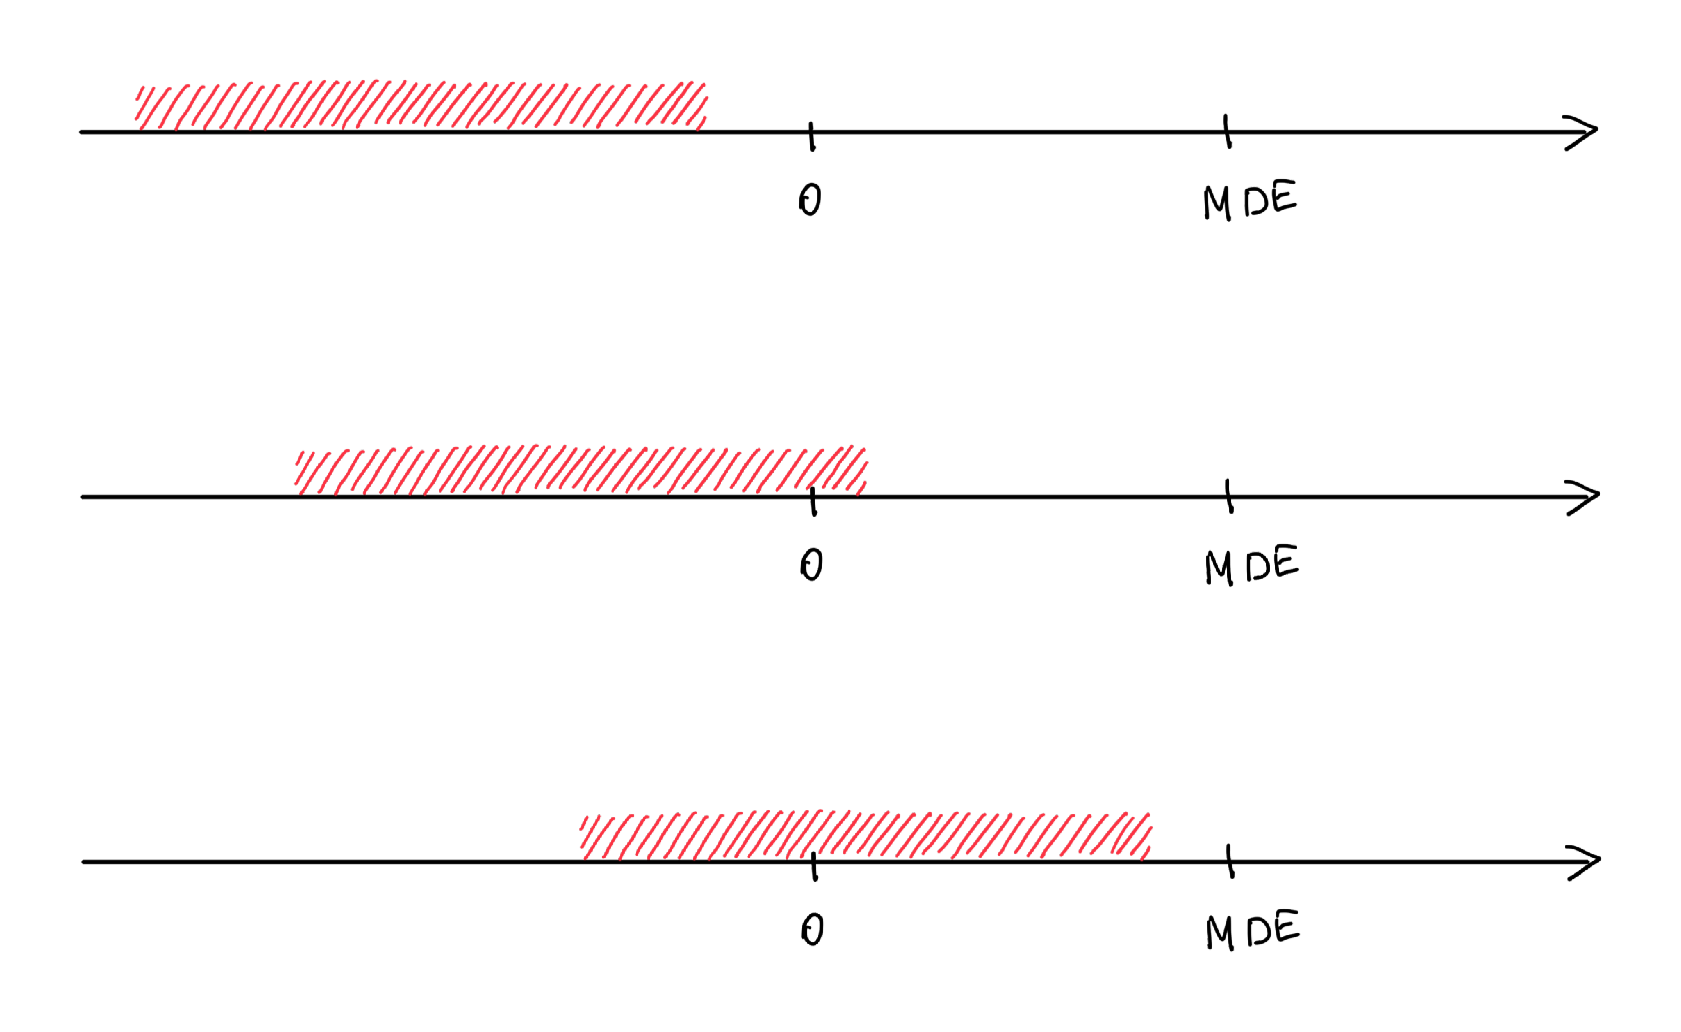
\includegraphics[width=1.1\columnwidth]{ab-test-red.pdf}
    % \caption{Красный тест}
    % \label{fig:move_y}
\end{marginfigure}
Допустим мы построили доверительный интервал для оценки~$\delta$ и он лежит
полностью правее нуля, то есть эффект от эксперимента отрицательный. Мы не
добились желаемого эффекта и значит от фичи стоит отказаться.

Аналогично, если интервал покрывает ноль, но не затрагивает MDE. Получается мы
не видим стат.значимого отклонения от нуля, зато видим стат.значимое отклонение
от MDE. Фичу не стоит раскатывать.

\paragraph{Серый тест.}
\begin{marginfigure}
    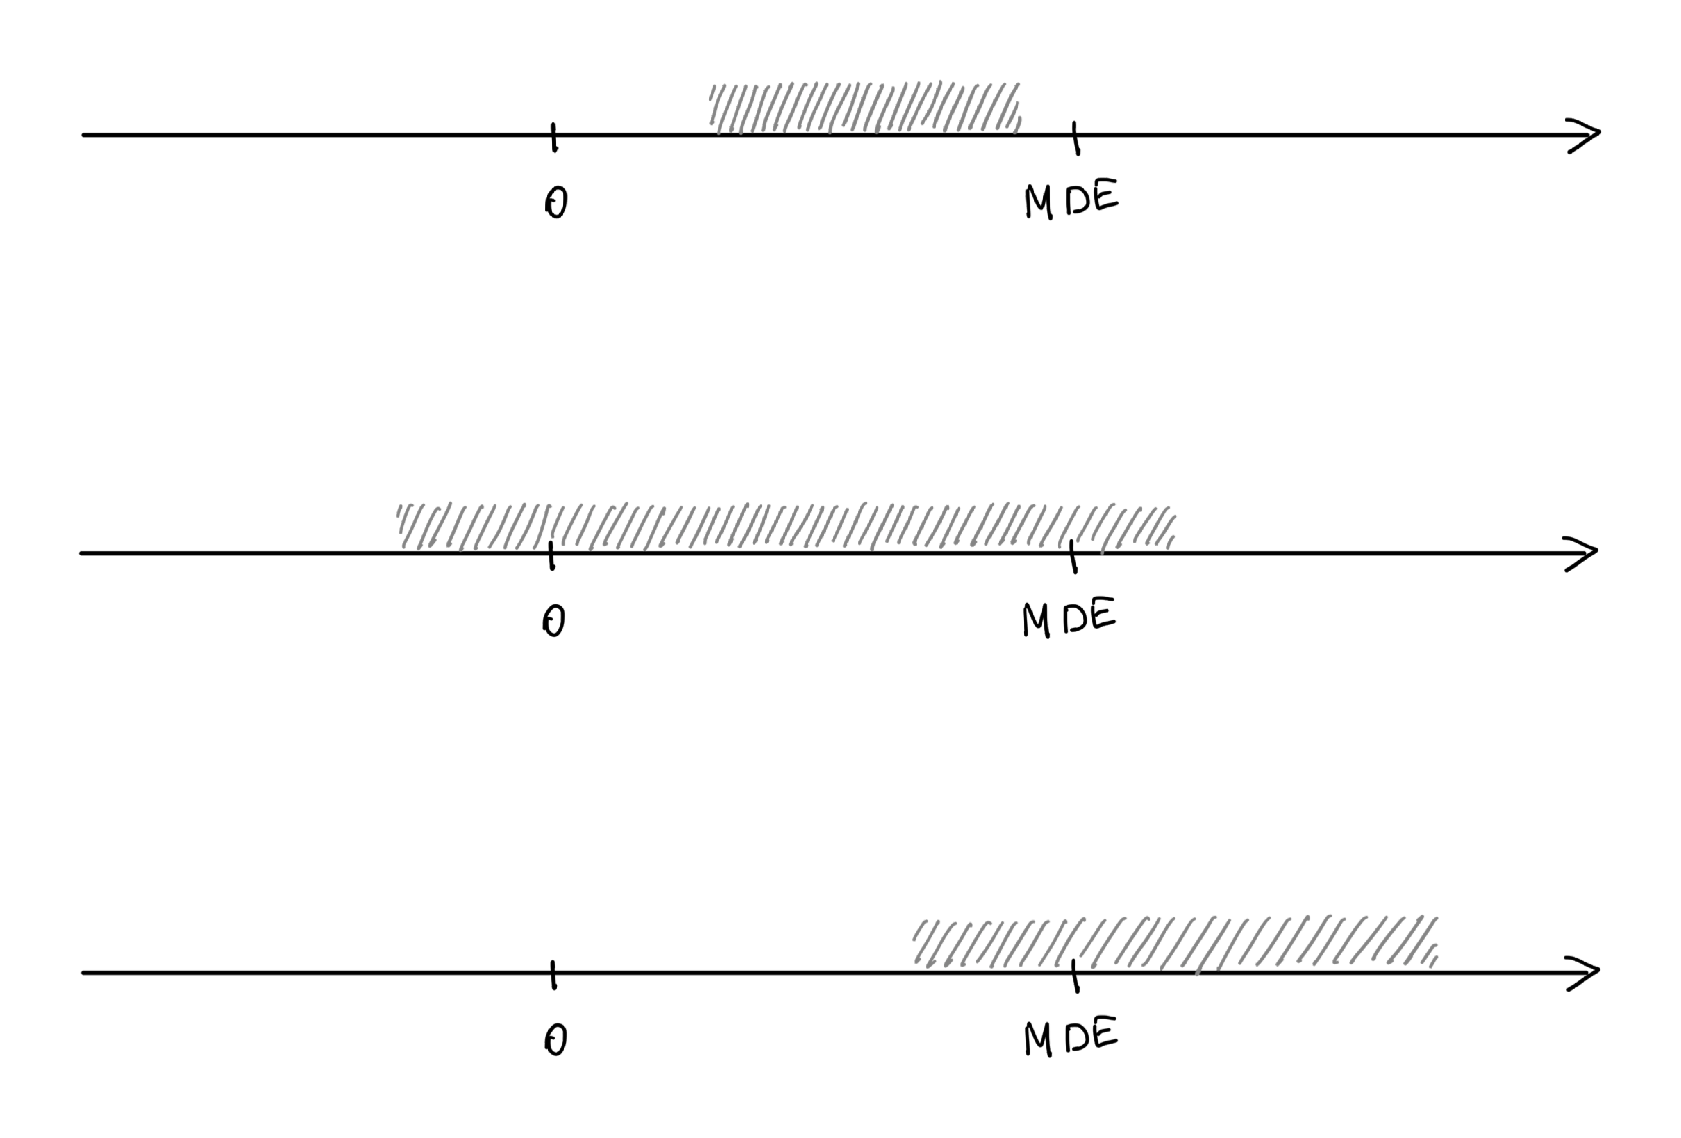
\includegraphics[width=1.1\columnwidth]{ab-test-gray.pdf}
    % \caption{Серый тест}
    % \label{fig:move_y}
\end{marginfigure}
Если доверительный интервал покрывает и 0 и MDE, это означает, что нет
стат.значимых отличий ни от нуля, ни от MDE. Видимо для теста нужно больше
времени. Здесь нужно смотреть по ресурсам, продление А/B-теста может
заблокировать другие эксперименты, а эффекта мы можем и не получить.

Возможна еще одна ситуация, когда у нас есть стат.значимые отличия и он нуля и
от MDE, но эффект который мы получили меньше, $0 < \delta < MDE$. В этом случае
тоже решение принимать стоит по обстоятельствам, эффект положительный, но ниже
наших затрат.

В случае если доверительный интервал покрывает MDE, но не покрывает ноля, мы
можем утверждать, что эффект положительный, но нет гарантий, что он превосходит
MDE, поэтому эксперимент стоит продлить, чтобы сделать более точную оценку
эффекта. Доверительный интервал должен сузиться на большем объеме данных и
возможно уже не будет покрывать MDE и сможем сделать более уверенные выводы.

\paragraph{Зеленый тест.}
\begin{marginfigure}
    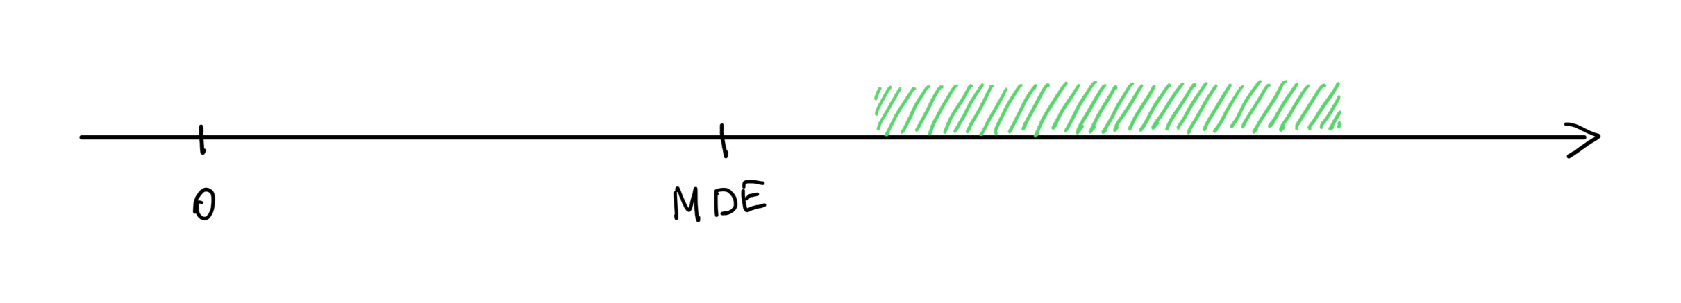
\includegraphics[width=1.1\columnwidth]{ab-test-green.pdf}
    % \caption{Зеленый тест}
    % \label{fig:move_y}
\end{marginfigure}
Если доворительный интервал полностью лежит правее MDE, значит мы достигла стат.значимого результата тест, можно принимать. Реальный эффект от внедрения фичи будет выше MDE.


\end{document}
